To support the key-value cache, each node must implement some form of indexing
service. Each indexing service must support a number of tasks such as
\emph{insertion}, \emph{deletion}, \emph{retrieval}, \emph{eviction} and
\emph{migration}. We consider three distinct but common indexing schemes:
\bptrees\cite{btree,bplustree}, Extendible Hashing\cite{ullman}, and
Counting Bloom Filters\cite{countingbloom1,countingbloom2}.

In order to operate in the elastic environment of our cache, when a node
overflows it must be capable of migrating a subset of its data records to
another node either preexisting or freshly allocated. Each of these schemes
have inherent differences in their structure and operation and, as such, are
compelling candidates for extension into the elastic makeup of \emph{Auspice}.

The remainder of this chapter will present background on each of the indexing
structures, describe the implementation of their migration mechanisms, and
provide an experimental analysis of their performance benchmarks.

\section{\bptrees} % (fold)
\label{sec:b_trees}
B-Trees and \bptrees are used in many of today's systems. The \bptree is a
multilevel indexing scheme that automatically adjusts the number of levels
depending upon the file size and stores all of its records in the leaf nodes.
Each record is stored in ascending order from left to right and each leaf node
is linked to the next and previous nodes. In this way, its design is
specifically crafted to accelerate queries over a range of
values\cite{navathe,ullman}. In terms of retrieval, \bptrees are balanced data
structures, where all paths from the root to any leaf have the same length
(similar to binary trees, with approximately log$_2 n$ depth).

\begin{figure}
\begin{center}
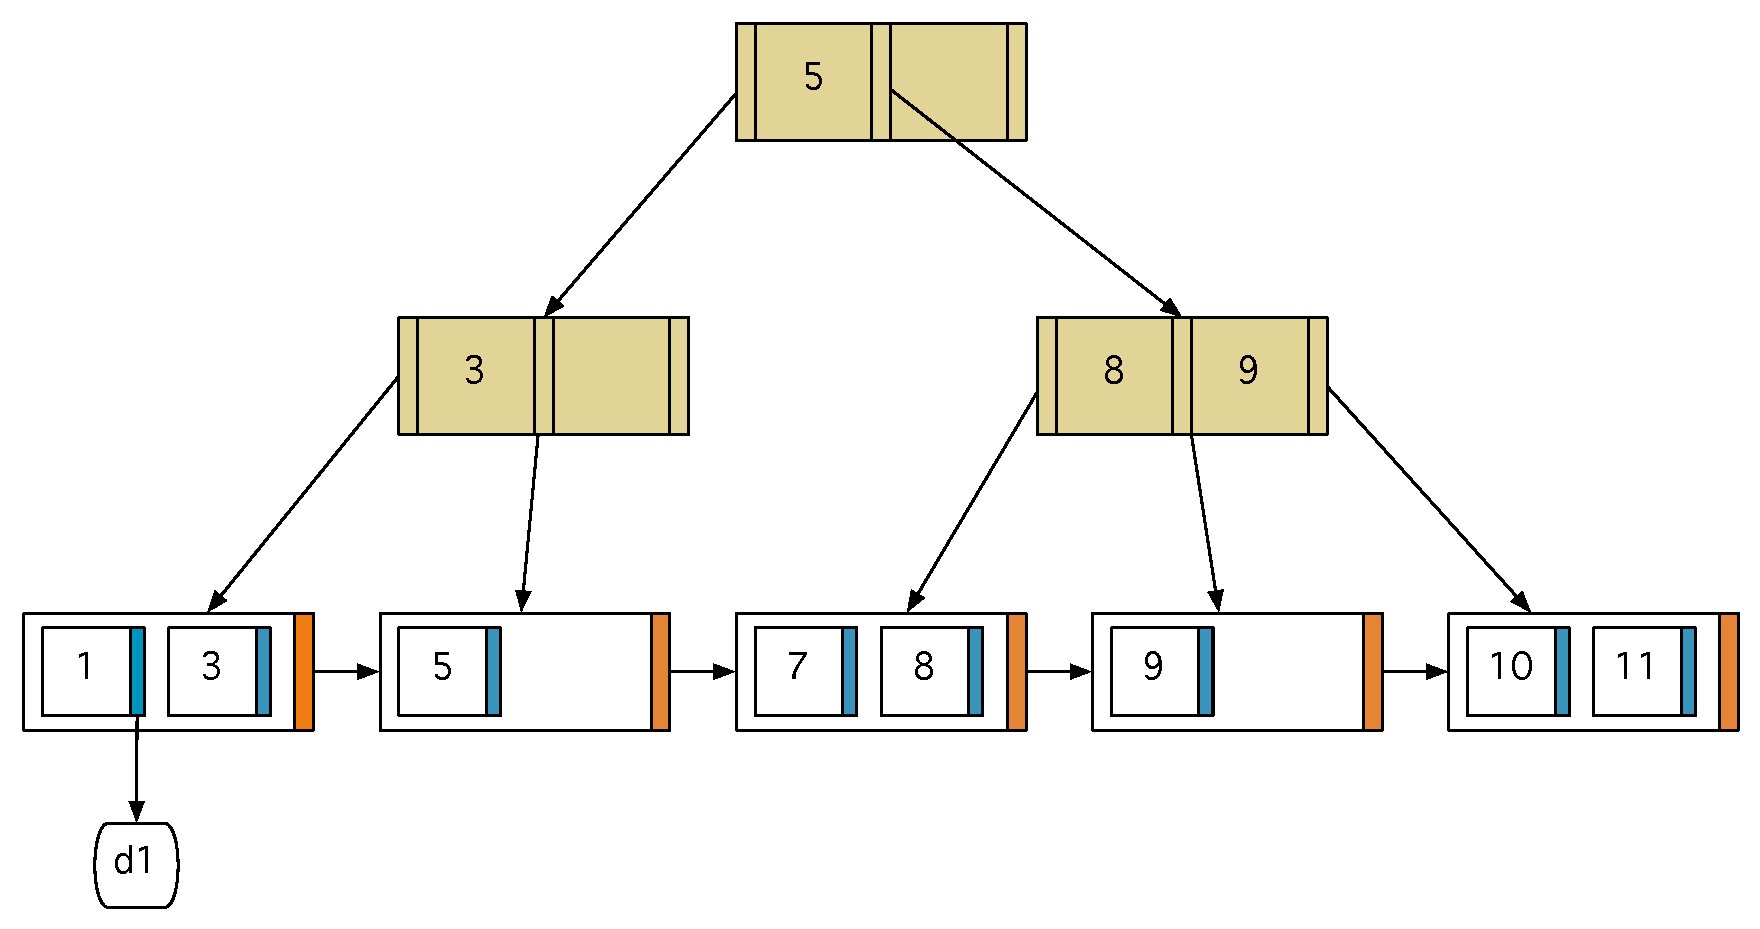
\includegraphics[scale=0.5]{figures/bplustree.pdf}
\end{center}
\caption{\bptree structure}
\label{fig:bplustree}
\end{figure}

Structurally, \bptrees are composed as shown in Figure~\ref{fig:bplustree}.
Internal nodes, those colored beige, act as pointers to other nodes in the
structure. All keys in the left branch of the key \emph{K} are less than or
equal to \emph{K}, while all keys to the right are greater than \emph{K}. While
searching, we compare the search key with the entries in the tree until such a
point as we reach the leaf node. Leaf nodes, those colored white, contain the
stored keys and pointers to the physical data location (blue). Additionally, in
order to assist with range queries, leaf nodes also contain a pointer to the
next leaf node, in order (orange).

With this sort of structure, we can see that range queries are made quite
simple and quick. Given a range $(k_{start}, k_{end})$ we begin by searching to
find $k_{start}$ then proceed to iterate through the leaves until we find a
node greater than $k_{end}$. The search then returns the set of data identified
in that range. Due to this support, we expect the \bptree integration to be
well suited to elastic cache. Quick access to ranges of data should lead to
much faster data migration in the event of node additions. Data migration,
which is composed of a set of key deletions, can again be efficiently managed
in the same way as a range query is.

% TODO: This section is cribbed heavily from IJNGC paper, look at rewrite.

% section B_Trees (end)

\section{Extendible Hashing} % (fold)
\label{sec:extendible_hashing}

% section extendible_hashing (end)

\section{Bloom Filters} % (fold)
\label{sec:bloom_filters}

% section bloom_filters (end)

\section{Experiments} % (fold)
\label{sec:experiments_indexing}

% section experiments_indexing (end)

\section{Results} % (fold)
\label{sec:results_indexing}

% section results_indexing (end)
